
All'interno dell'intensa campagna di studi condotta per verificare se le soluzioni previste per il progetto NUMEN possano garantire le prestazioni richieste, è stato svolto ad Aprile 2019 un test beam sui primi due prototipi di telescopi basati sulla tecnologia SiC-CsI.
Tale test si è tenuto ai Laboratori Nazionali del Sud (LNS) utilizzando un fascio di particelle di \ce{^{20}Ne} a 20~AMeV, prodotto dal Ciclotrone Superconduttore K800.
Al fine di favorire la generazione degli ioni di interesse per NUMEN, ovvero Ossigeno, Fluoro e Neon, si è scelto di utilizzare un bersaglio di \ce{^{12}C} da 400~$\mu$g/cm\ap{2}.


In questo capitolo vengono presentati i risultati ottenuti durante tale test e viene mostrato il confronto tra questi e i dati prodotti attraverso le simulazioni implementate per il presente lavoro di tesi. 
Dal momento che i prototipi utilizzati nel test presentano alcune differenze rispetto ai telescopi che verranno impiegati per NUMEN, è stato necessario modificare alcuni parametri della simulazione: in primo luogo, ricordando che, in uno dei due dispositivi (Tel~A), il primo stadio era montato in configurazione reverse, il substrato epitassiale del rivelatore al SiC è stato posto davanti al volume sensibile.
Inoltre, le dimensioni trasversali e gli spessori delle diverse componenti sono state cambiate in modo da riprodurre le caratteristiche descritte nel Paragrafo~\ref{par:telescopi}.


\section{\iflanguage{italian}{I dati del telescopio SiC-CsI}{Data of SiC-CsI telescope}}


Gli eiettili prodotti nell'interazione fra proiettile e bersaglio, dopo aver attraversato il quadrupolo e il dipolo, giungono al rivelatore di piano focale (Focal Plane Detector, FPD) di MAGNEX, dove, in occasione del test, erano stati posti i due telescopi, chiamati Tel~A e Tel~B. 
Come descritto nella Sezione~\ref{sez:test}, insieme ai due telescopi, erano stati montati quattro dei rivelatori al silicio attualmente in uso, i quali servivano da riferimento e da confronto per la Particle IDentification (PID).

Poiché all'energia utilizzata nel test i prodotti di reazione non erano in grado di superare il substrato epitassiale del Tel~B, da tale telescopio era possibile estrarre soltanto il segnale sulla perdita di energia, non permettendo di riprodurre le correlazioni $\Delta E - E_{resid}$ utili per l'identificazione in numero atomico $Z$ degli ioni.
Di conseguenza, dal momento che questo lavoro aveva lo scopo di studiare le performance di PID di tale sistema, sono stati analizzati soltanto i dati relativi al Tel~A.


%\subsection{\iflanguage{italian}{Le matrici $\Delta E_{SiC} - E_{CsI}$}{$\Delta E_{SiC} - E_{CsI}$ matrices}}

In Figura~\ref{fig:sic_csi_standard} è riportata la matrice $\Delta E_{SiC} - E_{CsI}$ registrata dal Tel~A utilizzando l'elettronica standard: come si può notare i luoghi dei diversi ioni appaiono ben separati in una regione che va dal Boro (B) al Neon (Ne).
Si può, inoltre, osservare che, poiché ai fini della PID non è necessario utilizzare la correlazione $\Delta E_{SiC} - E_{tot}$, i rivelatori non sono stati calibrati e, conseguentemente, le variabili $\Delta E_{SiC}$ e $E_{CsI}$ sono misurate in canali.


\begin{figure} [!p]
	\centering
	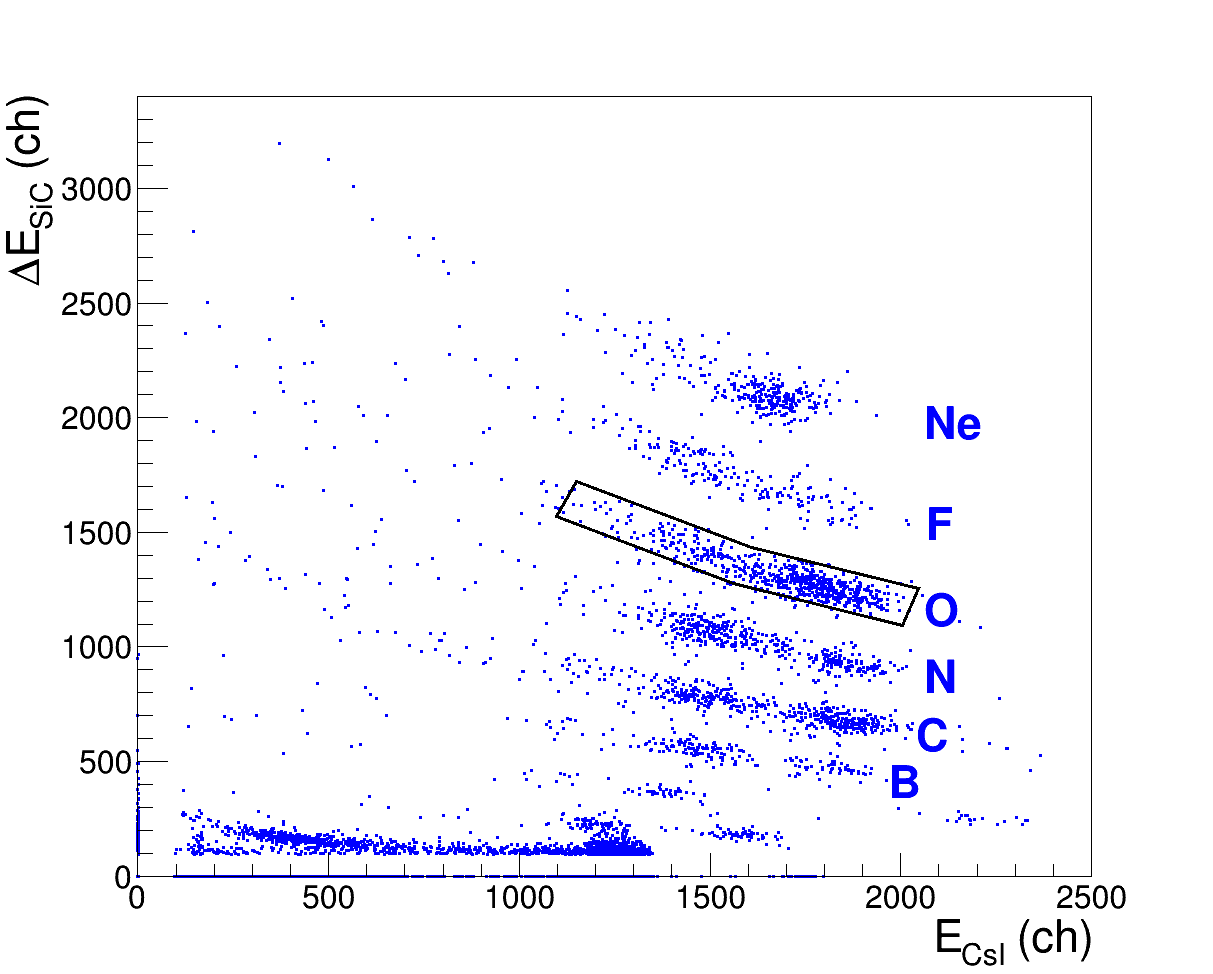
\includegraphics[width=\textwidth, keepaspectratio]{Grafici_Tesi/Test/matrice_sic_csi_taglio3.png}
	\caption{Le correlazioni $\Delta E_{SiC} - E_{CsI}$ ottenute dal Tel~A durante il test. La linea nera indica il taglio grafico effettuato per la selezione in numero atomico dell'Ossigeno.} \label{fig:sic_csi_standard}
\end{figure}

%Alla luce di questo risultato, il telescopio SiC-CsI sembra, dunque, rispondere alle richieste del progetto.
%Ricordando che questo telescopio era montato in configurazione reverse, si può anche osservare che il substrato epitassiale da 100~$\mu$m non sembra influire negativamente sulle sue proprietà di identificazione. 

%Ciò consente, dunque, di selezionare 

%Per confrontare le prestazioni di questo sistema con quelle solitamente ottenute utilizzando la co


%A questo punto può essere utile confrontare le prestazioni di questo sistema con quelle dell'apparato standard di MAGNEX, nel quale l'identificazione in numero atomico degli ioni avviene correlando la misura dell'energia persa $\Delta E$ nel gas con quella dell'energia residua $E_{resid}$ nei rivelatori al silicio; in particolare, la perdita di energia nel gas è data dalla somma delle sei perdite di energia $\Delta E_i$ misurate dai fili proporzionali.
%Inoltre, dal momento che la perdita di energia dipende dalla lunghezza della traiettoria dello ione all'interno del FPD, essa viene corretta, evento per evento, moltiplicando per il coseno dell'angolo di incidenza $\theta_{foc}$, ovvero 
%\begin{equation}
%	\Delta E^{corr}_{tot} \, = \, \frac{\cos \theta_{foc}}{\cos \theta_{tilt}} \, \sum_{i=1}^{6} \Delta E_i
%\end{equation}
%laddove $\theta_{tilt}$ rappresenta l'angolo di rotazione del FPD, pari a 59.2\textdegree.
In Figura~ si riporta la  matrice $\Delta E_{SiC} - E_{CsI}$ ottenuta con lo stesso telescopio utilizzando l'elettronica VMM3a: in questo caso si può notare che, sebbene si possano ancora riconoscere i luoghi corrispondenti ai diversi ioni, le curve sono parzialmente sovrapposte.
Ciò deriva da un maggiore contributo del rumore elettronico e da un peggiore accoppiamento fra i rivelatori e l'elettronica di front-end.
Dal momento che i dati relativi all'elettronica VMM3a non consentono un'agevole identificazione, si è scelto di analizzare soltanto quelli ottenuti utilizzando l'elettronica standard.



\section{\iflanguage{italian}{Analisi dei dati del test beam}{Analysis of test beam data}}

Per poter confrontare i dati sperimentali con i risultati delle simulazioni è necessario che queste riproducano nel modo più fedele possibile le condizioni sperimentali.
Dunque, è stata svolta un'analisi dei dati raccolti durante il test per estrarre delle informazioni da inserire opportunamente nella simulazione.
In primo luogo, è necessario stabilire quali ioni debbano costituire le particelle primarie nella simulazione, per cui è stata svolta un'identificazione dei prodotti di reazione.
%Inoltre, poiché l'energia delle particelle primarie è un parametro di fondamentale importanza, è stata determinare l'energia con cui gli ioni incidevano sul telescopio.
Inoltre, dal momento che un altro parametro di fondamentale importanza riguarda l'energia delle particelle, è stata condotta un'analisi per determinare l'energia di incidenza degli ioni sul telescopio.


%Ciò è stato possibile grazie alla correlazione tra posizione ed energia indotta dalla forza di Lorentz: 

\subsection{\iflanguage{italian}{Identificazione dell'\ce{^{16}O}}{Identification of \ce{^{16}O}}}

A causa della bassa statistica raccolta durante il test, è stato deciso di simulare soltanto la specie atomica più abbondante nel campione.
%, che, come si può evincere dalla Figura~, risulta essere l'Ossigeno.
La prima fase nella procedura di identificazione consiste nel determinare il numero atomico $Z$ delle particelle rivelate: tale informazione è stata ricavata dalle matrici $\Delta E_{SiC} - E_{CsI}$ in Figura~\ref{fig:sic_csi_standard}, dove si può notare che la specie atomica maggiormente presente è l'Ossigeno (O). 

Dopo avere selezionato gli ioni O è necessario distinguerne gli isotopi in numero di massa $A$; a tale scopo, si è sfruttata la correlazione tra posizione ed energia indotta dalla forza di Lorentz: ricordando la~\ref{eq:legge_spettrometri_approx}, è possibile notare che la correlazione $x_{foc} - E_{resid}$ permette di separare gli ioni in base al loro rapporto $\sqrt{m}/q$, laddove $m$ e $q$ rappresentano, rispettivamente, la massa e la carica della particella.
Nel caso del telescopio, la quantità $E_{resid}$ corrisponde con buona approssimazione a $E_{CsI}$.
La matrice $x_{foc} - E_{CsI}$ è mostrata in Figura~\ref{fig:xfoc2_csi_standard}, dove è possibile osservare che gli isotopi dell'O originati dall'interazione proiettile-bersaglio sono prevalentemente \ce{^{16}O}, \ce{^{17}O} e \ce{^{18}O}.
Si sottolinea che nella correlazione $x_{foc} - E_{resid}$ il numero di massa cresce spostandosi verso sinistra poiché, per mantenere lo stesso valore di $x_{foc}$, se la massa aumenta $E_{resid}$ deve diminuire.
Come si può notare dalla Figura~\ref{fig:xfoc2_csi_standard}, l'isotopo più abbondante dell'O presente nel campione è \ce{^{16}O}, la cui comparsa è probabilmente favorita poiché deriva da un processo di trasferimento di una particella $\alpha$ dal proiettile al bersaglio. 

\begin{figure} [!p]
	\centering
	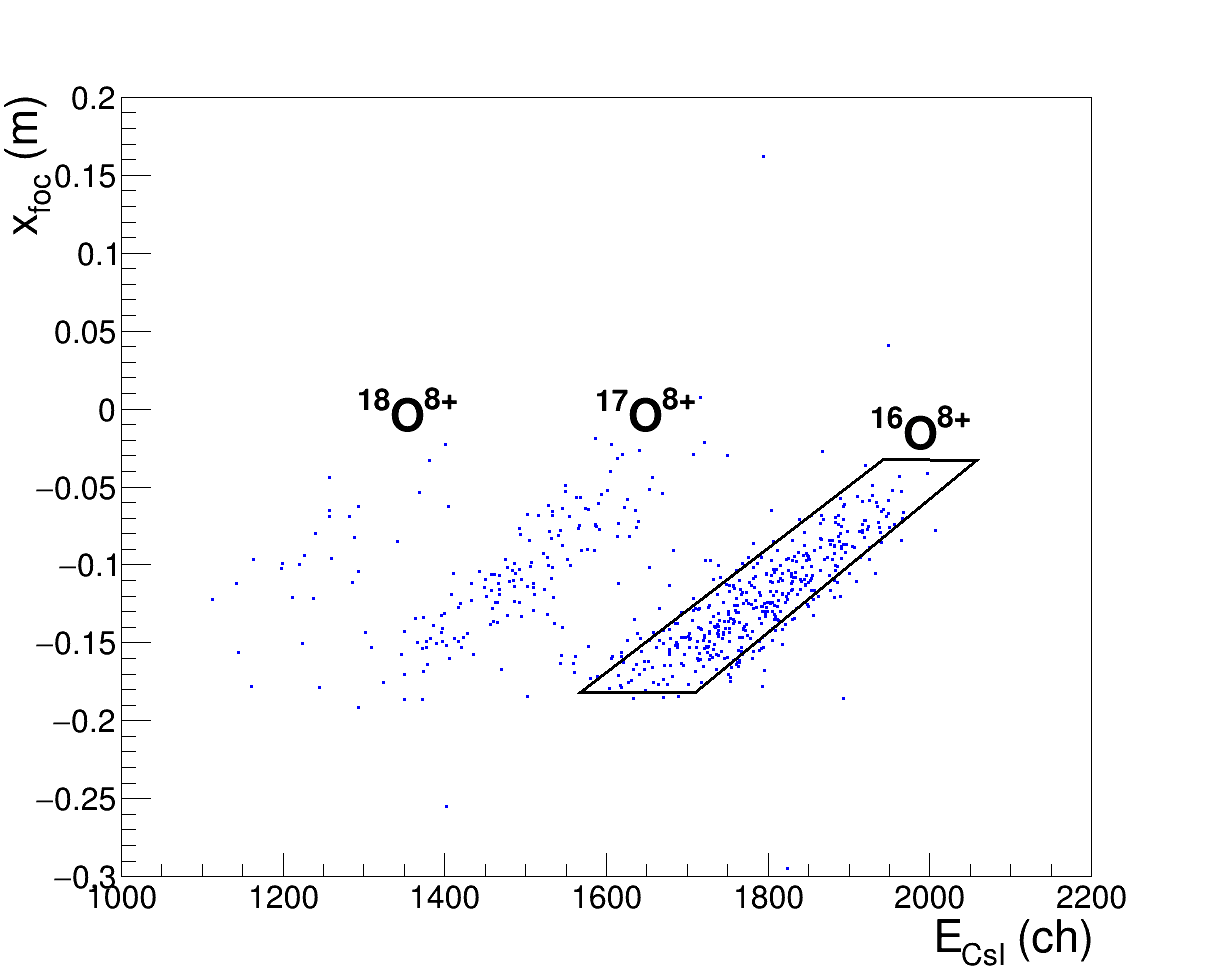
\includegraphics[width=\textwidth, keepaspectratio]{Grafici_Tesi/Test/matrice_xfoc2_csi_taglio.png}
	\caption{Le correlazioni $x_{foc} - E_{CsI}$ ottenute, durante il test, dalla misura in correlazione del tracciatore e del rivelatore allo CsI . La linea nera indica il taglio grafico effettuato per la selezione in numero atomico dell'\ce{^{16}O}.} \label{fig:xfoc2_csi_standard}
\end{figure}



\subsection{\iflanguage{italian}{Determinazione dell'energia dell'\ce{^{16}O}}{Energy determination of \ce{^{16}O}}}

Una volta identificato l'isotopo, è possibile determinare la sua energia cinetica $E_{kin}$ all'ingresso del rivelatore di piano focale (Focal Plane Detector, FPD) grazie alla correlazione tra l'angolo orizzontale $\theta_{foc}$ della traccia al piano focale e la coordinata orizzontale $x_{foc}$ del punto di arrivo della particella sullo stesso piano.
Ciascuno dei rivelatori di stop del FPD, indipendentemente dal fatto che si tratti di un rivelatore al silicio o di un telescopio, corrisponde ad una certa posizione $x_{foc}$; in particolare, dal momento che i rivelatori hanno superficie finita, ognuno di loro copre un'intervallo di posizioni in $x_{foc}$, legato alla propria estensione.
%Dunque, ricordando la~\ref{eq:legge_spettrometri_approx}, è possibile affermare che una misura di $x_{foc}$ equivale ad una misura dell'energia.
Dunque, ricordando la~\ref{eq:legge_spettrometri_approx}, è possibile affermare che, fissato lo ione, esso può arrivare in un certo intervallo in $x_{foc}$ soltanto con un determinato range energetico; in altre parole, gli ioni di \ce{^{16}O} che incidevano sul telescopio dovevano necessariamente avere degli specifici valori di energia.
Tali valori di energia sono correlati alle corrispondenti variabili $\theta_{foc}$ attraverso la cinematica della reazione $^{12}\mbox{C}\,  ( ^{20}\mbox{Ne}, ^{20}\mbox{O} ) \, ^{16}\mbox{O} $.

La matrice $\theta_{foc} - x_{foc}$ è riportata in Figura~\ref{fig:tefoc_xfoc2}, dove in rosso sono rappresentati i dati relativi al Tel~A, mentre in blu sono indicati i dati dello stesso ione, identificati tramite le tecniche di identificazione standard di MAGNEX.
\begin{figure} [!p]
	\centering
	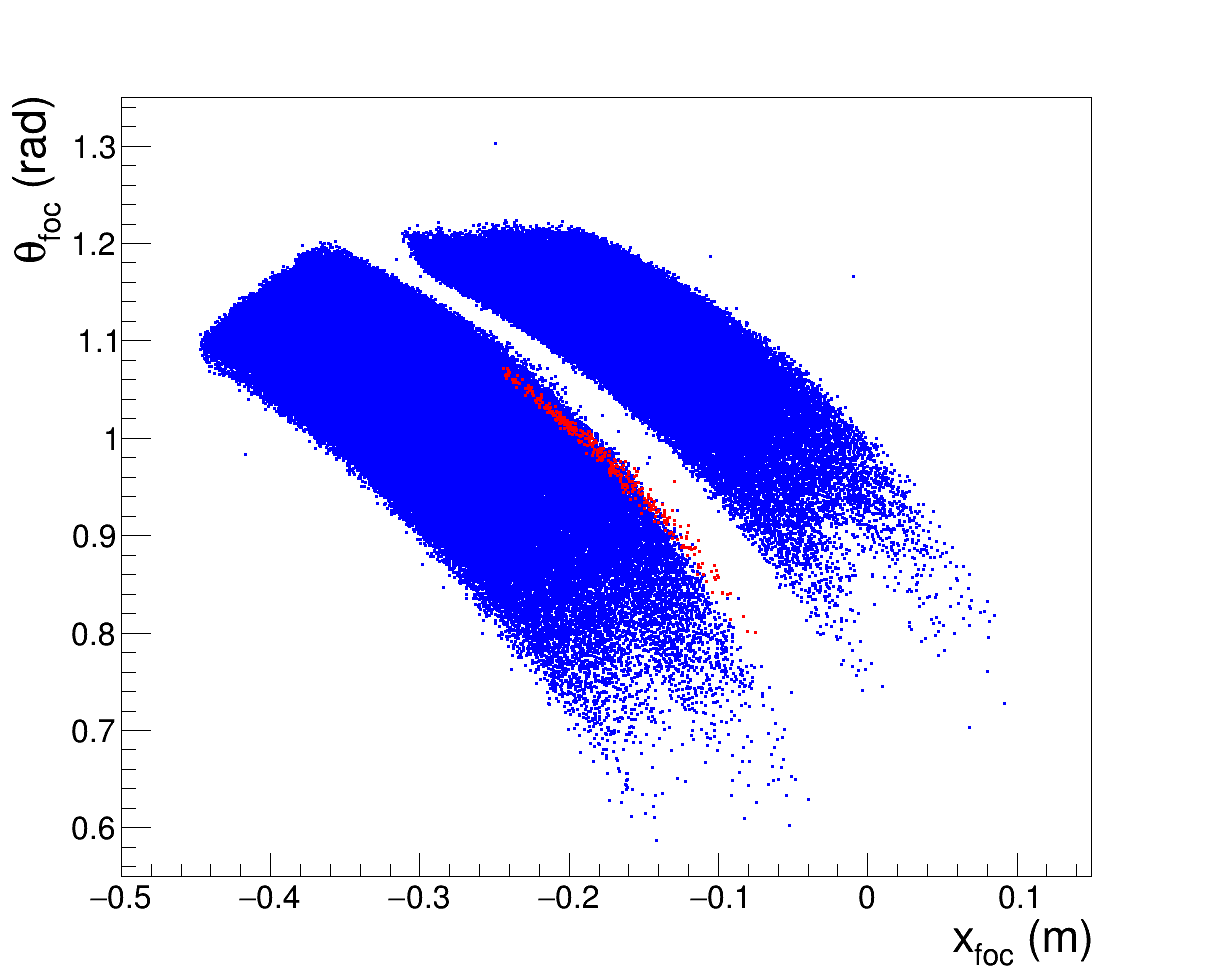
\includegraphics[width=\textwidth, keepaspectratio]{Grafici_Tesi/Test/matrice_tefoc_xfoc.png}
	\caption{Le correlazioni $\theta_{foc} - x_{foc}$ ottenute, durante il test, dalla misura in correlazione dell'angolo della traccia al piano focale e della posizione di arrivo allo stesso piano. Le matrici all'\ce{^{16}}: in blu sono riportati i dati misurati con i rivelatori standard di MAGNEX, in rosso sono mostrati i dati raccolti con il Tel~A.} \label{fig:tefoc_xfoc2}
\end{figure}
Come si può notare, la larghezza della striscia rossa è molto inferiore rispetto a quella delle strisce blu: ciò dipende dalla grande differenza fra la superficie del telescopio, pari a $1 \times 1$~cm\ap{2}, e quella dei rivelatori al silicio, ciascuna uguale a $5 \times 7$~cm\ap{2}.
In questo caso, le variabili $\theta_{foc}$ e $x_{foc}$ sono calibrate e sono misurate, rispettivamente, in radianti e metri.
Per determinare il range energetico all'interno del quale gli ioni di \ce{^{16}O} arrivavano sul telescopio, è sufficiente conoscere i valori di energia corrispondenti ai due estremi della striscia rossa.
Sebbene, in base a quanto detto, potrebbe sembrare possibile estrarre tale informazione a partire dalla sola misura della coordinata $x_{foc}$, in realtà, un punto della matrice $\theta_{foc} - x_{foc}$ potrebbe essere occupato da uno ione in uno stato eccitato.
È stata, quindi, svolta una simulazione, basata su metodi Monte Carlo, allo scopo di generare in modo casuale i parametri fisici dei prodotti della reazione in esame.
In tale simulazione sono stati presi in considerazione diversi stati eccitati dell'\ce{^{16}O} e, tramite una scelta accurata, si è fatto in modo che due di questi passassero per gli estremi della regione pertinente al telescopio.
Il risultato di tale procedura è mostrato in Figura~\ref{fig:simulazione}, dove, sovrapposti alle matrici precedentemente descritte, appaiono in nero i luoghi corrispondenti alle energie di eccitazione considerate.
\begin{figure} [!p]
	\centering
	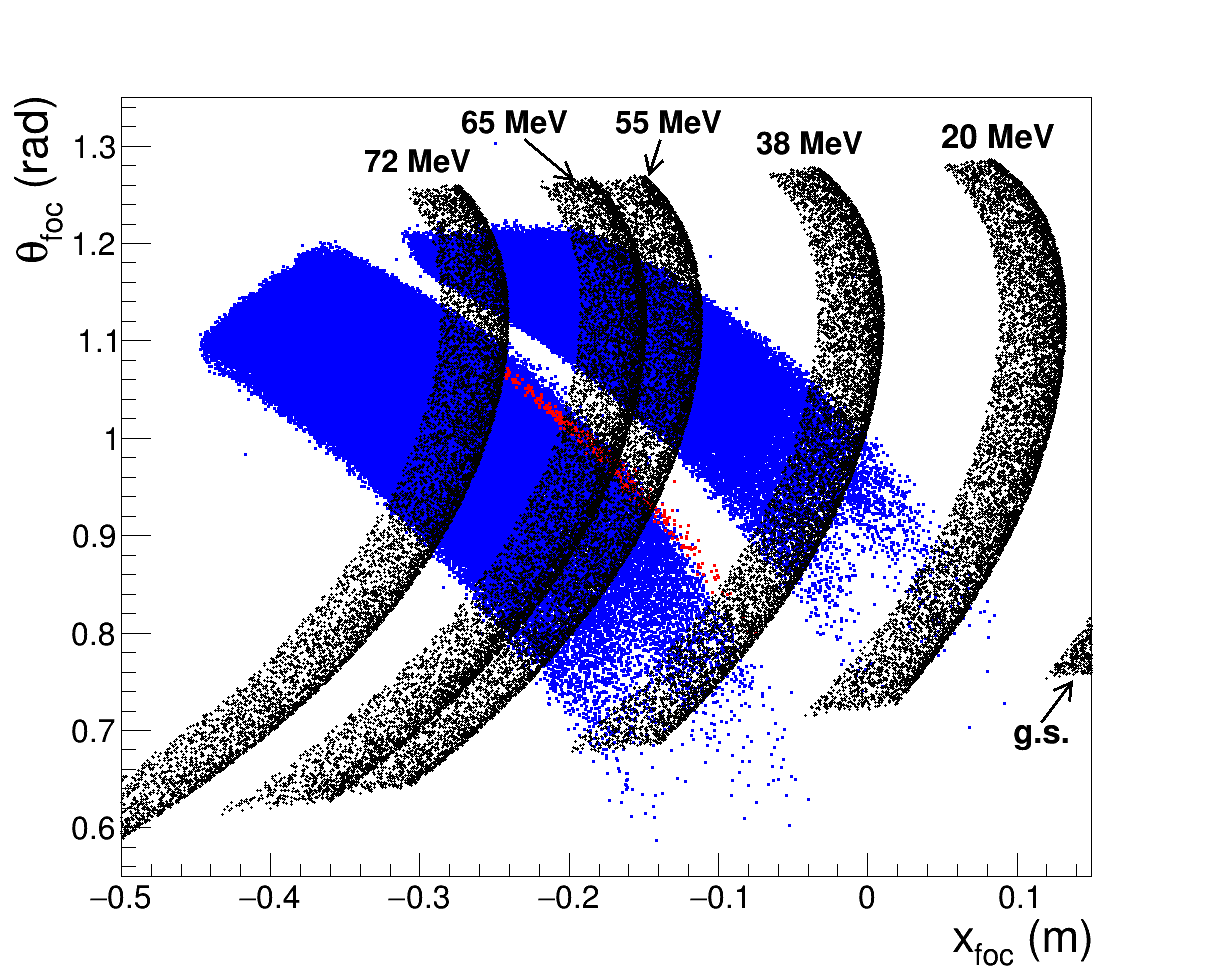
\includegraphics[width=\textwidth, keepaspectratio]{Grafici_Tesi/Test/simulazione.png}
	\caption{Il risultato della simulazione della reazione $^{12}\mbox{C}\,  ( ^{20}\mbox{Ne}, ^{20}\mbox{O} ) \, ^{16}\mbox{O} $ per diverse energie di eccitazione dell'\ce{^{16}O}.} \label{fig:simulazione}
\end{figure}
Come si può notare, gli ioni di \ce{^{16}O} si trovano in uno stato altamente eccitato, laddove gli estremi della regione del telescopio sono attraversati dagli stati eccitati a 38 e 72~MeV, mentre gli altri due stati a 55 e 65~MeV si posizionano circa a metà di tale regione.
%Nota questa informazione, si è utilizzato il software di cinematica CATKIN, grazie al quale, introducendo gli opportuni valori di energia cinetica del proiettile e di energia di eccitazione del l'eiettile, si è ricavata la correlazione l'energia cinetica dell'eiettile ad un determinato angolo di emissione.
%Nota questa informazione, per calcolare l'energia cinetica dell'eiettile si è utilizzato il software di cinematica CATKIN, nel quale vengono tenuti in considerazione i parametri rilevanti come energia di eccitazione e angolo di emissione. 
La simulazione permette, inoltre, di conoscere, evento per evento, l'energia cinetica dell'eiettile, nonché l'angolo di emissione $\theta_{p}$.
È bene sottolineare che tale angolo non coincide con $\theta_{foc}$, ma esiste una relazione empirica fra le due quantità, ovvero
\begin{equation}
	\theta_{p} = \frac{\theta_{foc} - \theta_{tilt}}{-2.7} + \ang{10}
\end{equation}
dove $\theta_{tilt}$ denota l'angolo di rotazione del FPD, $-2.7$ rappresenta l'ingrandimento angolare di MAGNEX e 10\textdegree{} indica l'angolo ottico dello spettrometro.
Prendendo in considerazione i quattro stati simulati è stato possibile ricavare quattro coppie $(\theta_{foc} , E_{kin})$, sulle quali è stato effettuato un fit lineare allo scopo di derivare una relazione fra le due grandezze.
La retta trovata ha la seguente equazione:
\begin{equation} \label{eq:correlazione_angolo_energia}
	\theta_{foc} \, = \, -0.012 \, E_{kin} + 4.588
\end{equation}

Grazie alla~\ref{eq:correlazione_angolo_energia} è possibile trasformare una misura di angolo in una misura di energia.
Dunque, gli eventi relativi al Tel~A nella matrice $\theta_{foc} - x_{foc}$ sono stati proiettati sull'asse verticale, ottenendo lo spettro energetico riportato in Figura~, il quale riproduce la distribuzione in energia cinetica degli ioni di \ce{^{16}O} all'ingresso del FPD.
Tali energie non corrispondono a quelle di incidenza sul telescopio, in quanto i prodotti di reazione devono prima attraversare la finestra di Mylar e il tracciatore a gas.
Sono state, quindi, calcolate le perdite di energia in queste due componenti grazie al software LISE++, variando opportunamente l'energia cinetica e l'angolo della particella.
Alla fine di tale procedura è stato possibile stimare che il range di energia con cui gli ioni di \ce{^{16}O} giungevano sul Tel~A era compreso tra 290 e 310~MeV.



\section{\iflanguage{italian}{Confronto fra i dati del test e la simulazione \geant}{Comparison between test data and \geant simulation}}

Noti tutti i parametri rilevanti, è stata svolta una simulazione per cercare di riprodurre lo spettro sperimentale. 
Dal momento che il processo di produzione degli ioni di \ce{^{16}O} nell'interazione fra proiettile e bersaglio è governato da una sezione d'urto che varia in funzione dell'energia, era necessario introdurre nella simulazione una ``modulazione'' del numero di particelle primarie generate rispetto all'energia.
A tal fine, si è eseguito un fit con un polinomio del quarto ordine sullo spettro in Figura~, ottenendo il risultato riportato in Figura~.
La distribuzione dell'energia cinetica delle particelle primarie deve, dunque, rispecchiare l'andamento di tale funzione di fit.
Nella simulazione si è provato ad ``imitare'' la sezione d'urto della reazione definendo una variabile che svolgesse il ruolo di probabilità del processo.
Venivano, dunque, estratte in modo casuale ed uniforme l'energia della particella nel range compreso tra 290 e 310~MeV 

